\section{Testing the effect of a \kpi S-wave}
\label{sec:swave:testing}

In an angular analysis of \BdToKpill, the S-wave can be considered to be 
a systematic effect that could bias the results of the angular observables.
The implications of this systematic effect are tested by generating toy 
Monte Carlo experiments and fitting the angular distribution to them.
The results of the fit to the observables are evaluated for multiple toy 
datasets.

The effect of the S-wave is evaluated for two different cases.
Firstly, the effect of S-wave interference  is examined as a function 
of the size of the dataset used.
The aim of this study is to explore the possibility of biases in any measurements to date and the
 possible implications on future measurements of \BdToKpill.
Datasets of sizes between 50 and 1000 events are tested.
For comparison, the results from Chapter~\ref{chap:kstmm} 
have between 20 and 200 signal events in the 6 different \qsq bins considered.
Second, the effect of different levels of S-wave contribution is examined. 
At present, the only information about the S-wave fraction is 
obtained by the measurement of \FS of approximately 7\% in the decay $\Bd\to\jpsi\kpi$
from~\cite{Aubert:2004cp} for the range $800 < p < 1000 \mev$. 
As the value may be different in \BdToKpill, we consider 
values of \FS in this region ranging from 1\% to 60\%. 
The fraction of the S-wave, \FS, is expected to have some \qsq dependence
 because of the \qsq dependence of the transverse P-wave amplitudes.

The parameters used to generate the toy datasets are summarised in 
Tables~\ref{tbl:params} and~\ref{tbl:obs}.
The values of the angular observables used  to generate toy Monte Carlo
 simulations are taken from the analysis of 1.0\invfb presented in~\cite{LHCb-CONF-2012-008}. %Section~\ref{sec:kstmm:results}.
Within errors, these measurements are compatible with the Standard Model prediction for \BdToKstll 
and the central value of the measurement is used.
The nominal magnitude  and phase difference of the S-wave contribution 
are taken from the angular analysis of \Bd\to\jpsi\kpi~\cite{Aubert:2004cp}.
The toy datasets are generated as samples of pure signal in order to test the
trend on the bias on the angular observables in the signal distribution that could be incurred from an increasing \kpi S-wave component.
As this is a phenomenological study, a background component is not included as this is not expected to affect the trends.
The correlation between the S-wave component and any possible background is expected to be small. This
expectation is based on the results presented in Table X of~\cite{LHCB-PAPER-2013-002} where the uncertainty in the background on the \Kp\Km S-wave component in
the \Bs\to\jpsi\varphi final state is evaluated and shown to be small.
\begin{table}[tb]
\caption[ Parameters used to generate toy datasets.   ]
{Parameters used to generate toy datasets. \AFB, \FL, \AT2 and \AIm
 are taken from ~\cite{LHCb-CONF-2012-008} %Section~\ref{sec:kstmm:results}  
 in the $1 < \qsq < 6~(\gev^2)$ bin. 
The \FS value is taken from Ref.~\cite{Aubert:2004cp}~\label{tbl:obs}}.
\centering
\begin{tabular}{|c|c|c|c|c|c|}
\hline
Obs.  & \AFB & \FL & \AT2 & \AIm  & \FS  \\
\hline
Value &$ -0.15 $ &$ 0.65$  & $ 0.03/(1-0.65)$ & $0.05$  & $0.07$  \\
\hline
\end{tabular}
\end{table}

The toy datasets are generated as a function of the
 \ctl, \ctk, $\phi$ and \psq using an accept/reject method.
 The PDF used is the angular distribution given in 
 Eq.~\ref{eq:theo5d}.
For each set of input parameters 1000 toy datasets were generated.
For each of these toy datasets, an unbinned log likelihood fit is 
performed that returns the best fit value of the observables 
and an estimate of their error.
The expected experimental resolution is obtained by plotting 
the best fit values of an observable for the ensemble of toy 
simulations as illustrated for \AFB in Fig.~\ref{fig:toyexample} (left).
 The pull value for an observable ($O$) is defined as 
\begin{align}
p_{O}^i= \frac{ O_{\text{fit}}^i - O_{\text{gen}}^i }{ \sigma_{O}^i }
\end{align}
where $\sigma_O^i$ is the estimated error on the fit to the observable $O^i$.
This distribution is seen in Fig.~\ref{fig:toyexample} (right). 
The mean and the width are extracted from a Gaussian fit.
For a well performing fit without bias, the pull distribution should 
have zero mean and unit width. 
A negative pull value implies that the result is underestimated 
and a positive pull value implies overestimation of the true observable.
\begin{figure}[tb]
\centering
\subfigure[]{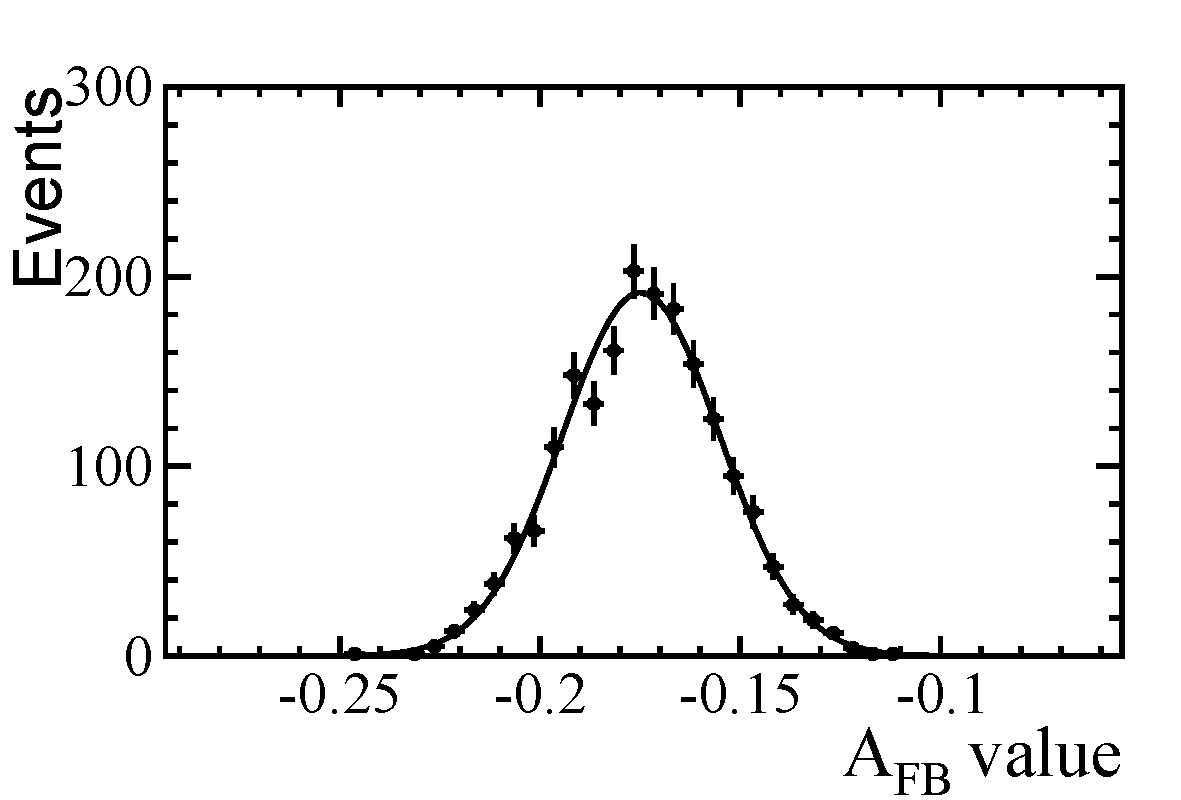
\includegraphics[width=0.48\textwidth]{chapter6/figs/fit_result_test_afb_gen_val_plot_new.pdf}}
\subfigure[]{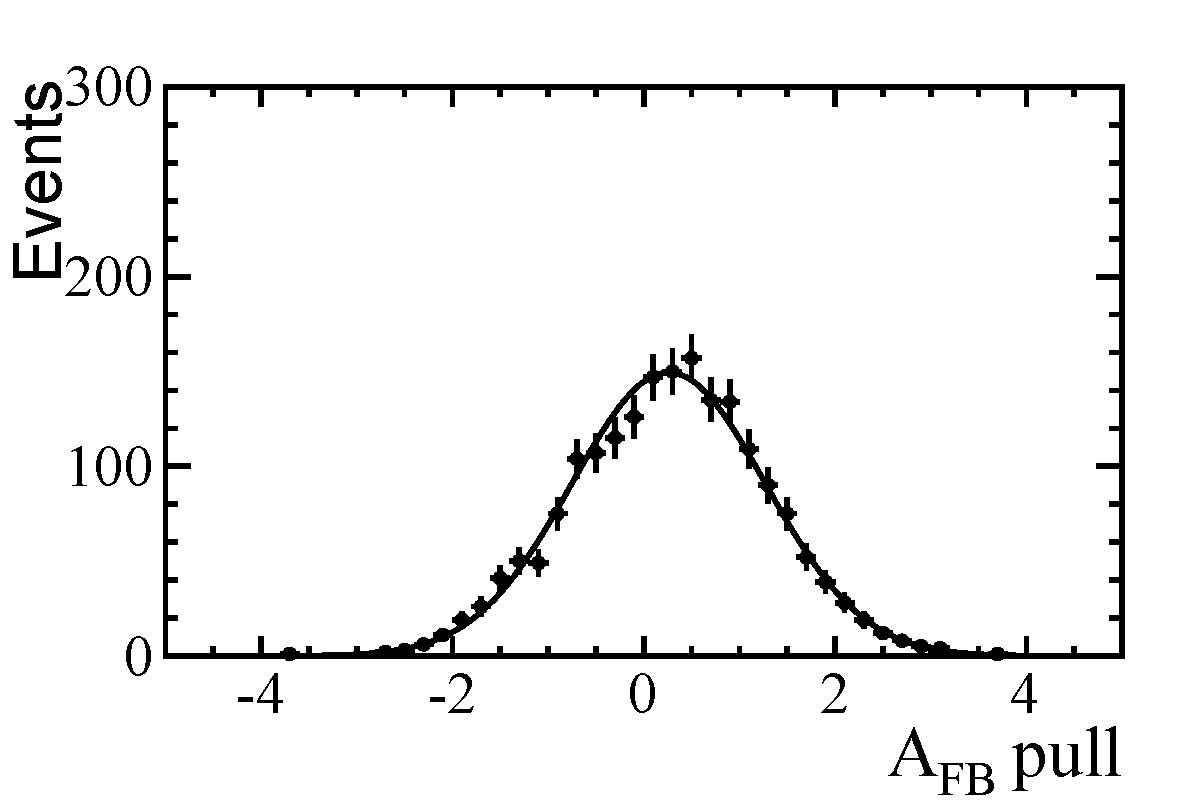
\includegraphics[width=0.48\textwidth]{chapter6/figs/fit_result_test_afb_gen_pull_plot_new.pdf}}
\subfigure[]{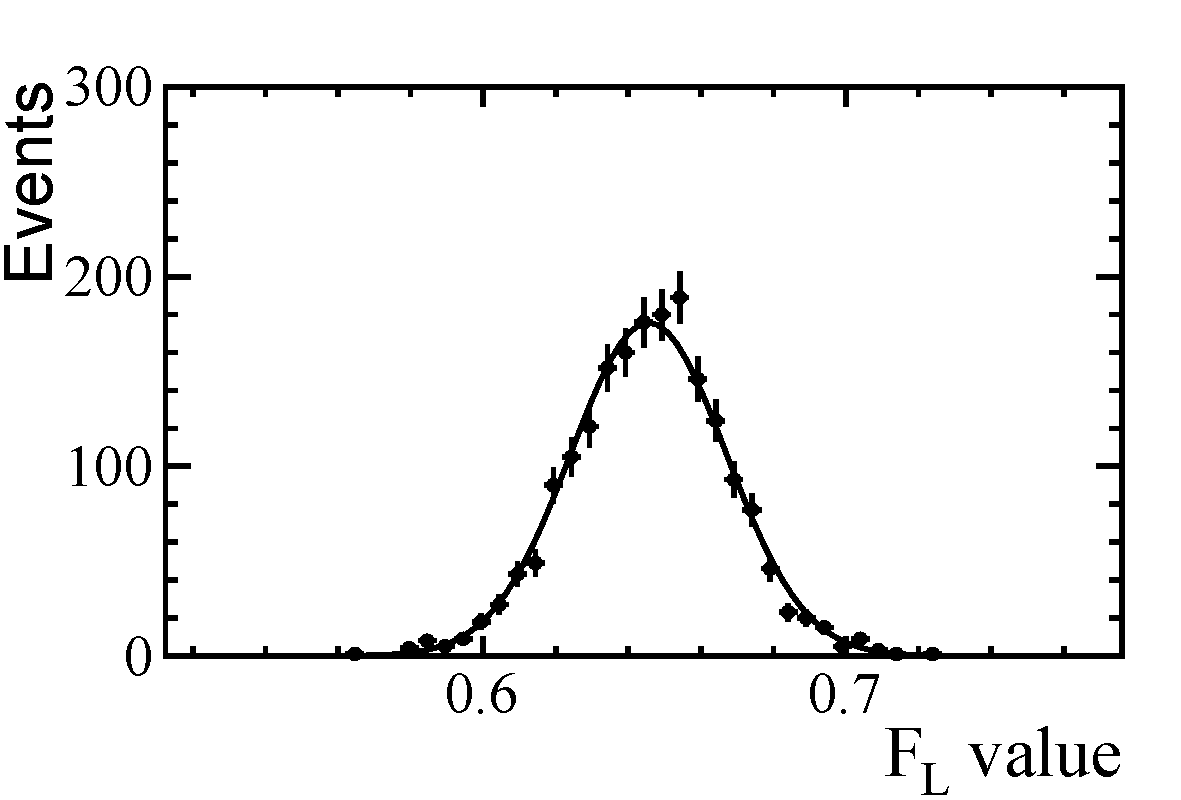
\includegraphics[width=0.48\textwidth]{chapter6/figs/fit_result_test_fl_gen_val_plot_new.pdf}}
\subfigure[]{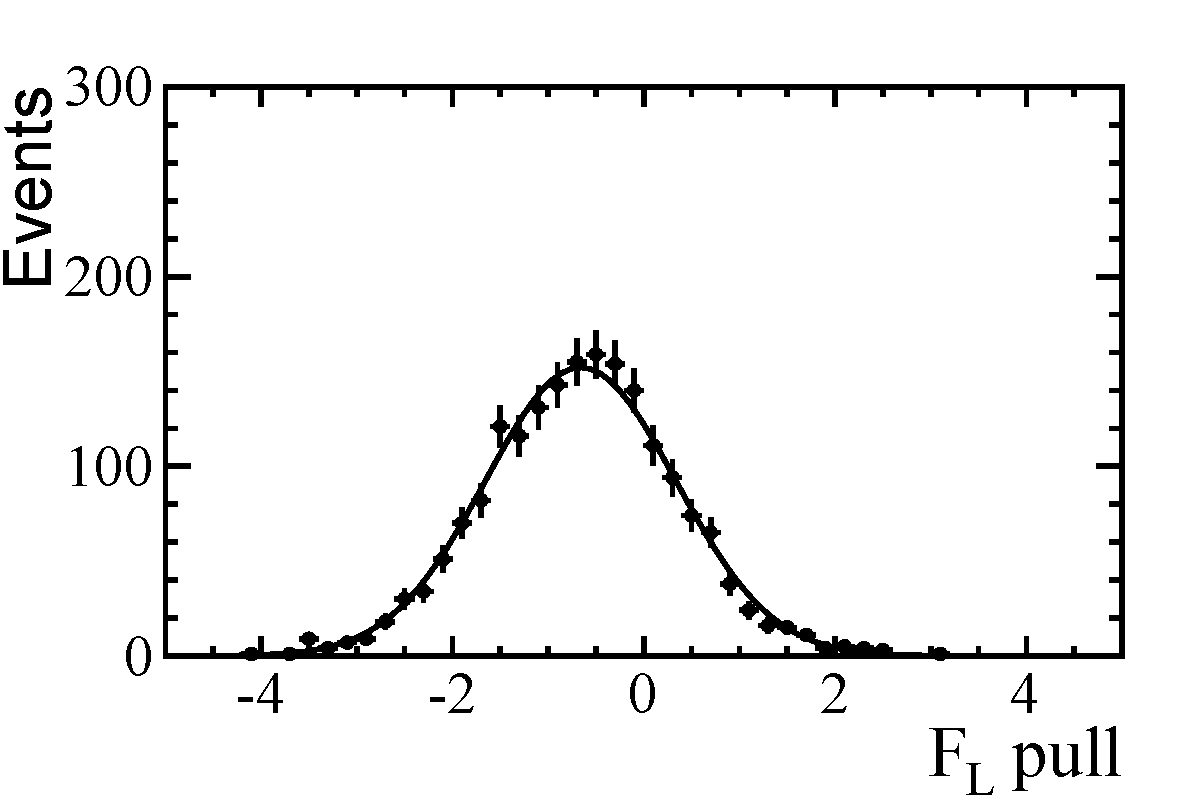
\includegraphics[width=0.48\textwidth]{chapter6/figs/fit_result_test_fl_gen_pull_plot_new.pdf}}
\caption[  Distribution of the results and pull  
values for \AFB (a,b) and \FL (c,d) respectively 
for fits to 1000 toy simulations each containing 1000 events. ]
{Distribution of the results and pull 
values for \AFB (a,b) and \FL (c,d) respectively 
for fits to 1000 toy simulations each containing 1000 events.
The S-wave is ignored in these fits. The resolution obtained on \AFB is 
$0.026\pm0.001$. Since the S-wave is ignored there is a non-zero 
pull mean for both observables at $(0.26\pm0.02)$ and $(-0.65\pm0.02)$ respectively. 
The widths of the pull distribution are consistent with unity at 
 $(1.01\pm0.01)$ and $(0.99\pm0.01)$.~\label{fig:toyexample}}
\end{figure}

